%% ---------------------------------------------------------------------------
%% Auto-Echo -- MSc dissertation research paper (QMUL EECS, 2025-26)
%%
%% Format fixed by the MSc Project Guide Sec. 4.3.1: IEEEtran, two columns,
%% 12 pages EXCLUDING references and appendices. See PAGE_BUDGET.md.
%%
%% NOTE: the formative (9 July) draft this replaces is preserved as
%% Formative_Draft_9July.tex.bak and in git. It describes the SUPERSEDED
%% sample-based probe; nothing in it should be reused without checking it
%% against the final WSS pointer-chase methodology.
%%
%% Two constraints that are easy to get wrong, both established by testing:
%%
%%  1. REFERENCING. Guide Sec. 8.1: "The Faculty of Science and Engineering at
%%     QM requires students to use the Harvard system ONLY." IEEEtran defaults
%%     to numbered citations, so natbib is loaded in author-year mode and the
%%     bibliography is hand-written as \bibitem[Label(Year)]{key}. BibTeX is
%%     deliberately NOT used: the guide's worked examples have no comma before
%%     the year and no full stop after "et al", and no stock .bst emits either.
%%
%%  2. UNICODE. pdflatex + T1 SILENTLY DROPS U+2713, U+2717, U+2212 and U+2248
%%     -- no error is emitted and the glyph simply does not appear in the PDF.
%%     Verified by compiling a torture-test document: zero warnings, missing
%%     output. Use \cmark, \xmark, $-$ and $\approx$. Never paste those
%%     characters into this file.
%% ---------------------------------------------------------------------------
\documentclass[conference]{IEEEtran}
\IEEEoverridecommandlockouts

\usepackage{amsmath,amssymb,amsfonts}
\usepackage{graphicx}
\usepackage{textcomp}
\usepackage{booktabs}
\usepackage{array}
\usepackage{url}
%% NB: multirow and threeparttable are NOT installed in this TeX Live scheme.
%% Do not add them without checking `kpsewhich multirow.sty` first -- an
%% examiner rebuilding this on a stock installation would hit a hard failure.

%% --- Harvard citations (Guide Sec. 8.1) ------------------------------------
%% aysep={} drops the comma between author and year, giving "(Leyden 2005)"
%% exactly as the guide's worked example shows.
\usepackage[round,authoryear]{natbib}
\setcitestyle{aysep={}}
\bibliographystyle{plainnat}

%% --- Glyphs pdflatex cannot take as literal Unicode ------------------------
\newcommand{\cmark}{\ensuremath{\checkmark}}
\newcommand{\xmark}{\ensuremath{\times}}

\begin{document}

\title{Auto-Echo: Automated Discovery of Cache-Hierarchy\\
Structure from User-Space Latency Alone}

\author{\IEEEauthorblockN{Harsh Raj Singh}
\IEEEauthorblockA{\textit{MSc Advanced Computer Science} \\
\textit{Queen Mary University of London}\\
London, United Kingdom \\
ec25303@qmul.ac.uk}}

\maketitle

\begin{abstract}
Can a program discover its machine's cache hierarchy --- how many levels it has
and how large each is --- from timing alone, with no privileges, no vendor tables
and no architecture-specific instructions? The usual answer is to read a table
somebody else has filled in, but that table can be incomplete, and it can be
complete and still not describe how the machine behaves. This paper presents
Auto-Echo, which answers the question by measurement. A flush-free pointer-chase
probe with batch-amortised, runtime-calibrated timing produces a
latency-versus-working-set-size curve; an unsupervised stage then determines the
hierarchy from it, with exact one-dimensional clustering counting the memory
levels and count-constrained change-point detection localising each capacity. No
threshold, penalty or level count is supplied anywhere in the productive path,
and the counting step is solved to global optimality by dynamic programming
rather than by a local-search heuristic, making it deterministic. On an Apple M1
and an Intel Core i5-13450HX the same code path recovers every documented cache
within a factor of two --- 2/2 and 3/3 respectively, at 100\% precision ---
against operating-system ground truth that is itself cross-checked against an
independent implementation. Two boundary conditions are established by controlled
experiment rather than asserted. Page size, not cache size, decides whether a
last-level cache is visible at all: the Intel machine's documented 20\,MiB L3 is
behaviourally unreachable under default 4\,KiB pages and resolves at 19.7\,MiB
only under a 2\,MiB huge-page allocation. And what a single core recovers of a
\emph{shared} cache is not its capacity but the share left to it, which an
eight-core streaming load drives down by a factor of five. The M1 result includes
a cache no operating-system interface reports.
\end{abstract}

\begin{IEEEkeywords}
cache hierarchy, memory latency, performance measurement, unsupervised learning,
change-point detection, computer architecture
\end{IEEEkeywords}

%% ===========================================================================
\section{Introduction}
\label{sec:intro}
%% TARGET 900 words / 1.1 pages

Every program's performance depends on the shape of the cache hierarchy it runs
on: how many levels exist, and how large each one is. Wulf and McKee's ``memory
wall'' \citep{wulf1995} named the structural cause --- processor and memory
speeds improving at different exponential rates --- and Drepper's
practitioner survey \citep{drepper2007} draws the corollary that performance on
modern hardware is largely decided by how a program's working set maps onto that
hierarchy. Knowing the hierarchy's shape is therefore a precondition for
reasoning about performance, yet the shape itself is largely opaque to
unprivileged software.

The standard response is to consult a table that somebody else has already filled
in. Three sources dominate, and it is worth being precise about what each
actually is, because the case for measurement is easy to overstate. The first is
the \emph{commercial} view: the vendor's own system report. The second is the
\emph{software} view: the operating system's cache descriptors, read through a
library such as \texttt{hwloc} \citep{broquedis2010}, an architecture-specific
instruction such as the x86 \texttt{CPUID} deterministic cache-parameter leaf
\citep{intel2023}, or a vendor tool such as Intel's Memory Latency Checker
\citep{intel_mlc}. The third is measurement.

This paper reports what the same two machines --- an Apple M1 and an Intel
Core i5-13450HX --- look like through all three lenses, and the three do not
agree.

The commercial lens is the one most users ever consult, and on both machines it
reports the processor, its core count and its installed memory, and \emph{not one
figure about the cache hierarchy}. Anyone who needs the size of L1 has already
been forced to a second tool.

The software lens is that second tool, and on hardware whose vendor filled in the
table it is excellent. On the Intel machine \texttt{lstopo} reports a complete and
correct hierarchy --- 48\,KiB L1d and 1280\,KiB L2 per performance core, a
20\,MB shared L3 --- which independent measurement then confirms. Nothing here
disputes that, and an argument for measurement resting on the descriptor being
\emph{inaccurate} would simply be false. Its limitation is narrower and more
interesting: its chain of trust terminates at what the operating system was told,
so it inherits the firmware's omissions exactly.

That limitation bites in two distinct ways, and this work exists because of both.

\textbf{The table can be incomplete.} On the Apple M1, \texttt{lstopo} reports the
128\,KB L1d and the 12\,MB L2 and then stops. The System-Level Cache is absent
--- not misreported, \emph{absent} --- because Apple exports it through no
interface \texttt{hwloc} can read. Section~\ref{sec:eval} shows the probe
responding to capacity well beyond the documented 12\,MB L2, resolving the L2 and
the SLC as a single 13.9\,MiB band. What was never written down cannot be looked
up; it can only be measured.

\textbf{The table can be complete, yet topology is not behaviour.} On the Intel
machine \texttt{lstopo}'s 20\,MB L3 is entirely correct as a statement about the
silicon --- and under the default 4\,KiB page size that L3 is behaviourally
\emph{unreachable}. Past roughly 1.3\,MiB the measured curve climbs and saturates
at a flat ${\sim}143$\,ns plateau by 4--5\,MiB, because once the working set
outruns the translation lookaside buffer's reach every dependent load triggers a
page-table walk that itself misses to DRAM. The cache is present; the machine
cannot reach it before translation cost dominates. A 2\,MiB huge-page allocation
lifts the masking and the same code path then recovers the L3 at 19.7\,MiB, within
$-1.5\%$ of nominal.

The second case is the sharper of the two, because no descriptor is wrong in it. A
table reports what a cache \emph{is}; it cannot report what a workload can
\emph{use}, and the gap between those is a property of the running system ---
page size, TLB reach, and, as Section~\ref{sec:eval} shows under load, how much of
a shared cache the other cores have left. Measurement is therefore not a less
accurate substitute for the descriptor. It answers a different question.

\textbf{Contributions.} This paper makes four.

\begin{enumerate}
\item A portable, flush-free working-set-size pointer-chase probe with
batch-amortised timing and a tick-to-nanosecond conversion \emph{calibrated at
runtime}, removing any dependence on a configured CPU frequency
(Section~\ref{sec:method}).
\item An automatic, penalty-free level-discovery stage in which clustering
\emph{counts} the memory levels and change-point detection \emph{localises} each
capacity, with the counting step solved to global optimality by dynamic
programming rather than by Lloyd's heuristic (Section~\ref{sec:method}).
\item A self-validating evaluation on two real ISAs, in which every documented
cache on both machines is recovered and matched against operating-system ground
truth that is itself cross-checked against an independent implementation
(Section~\ref{sec:eval}).
\item Two measured boundary conditions on what user-space discovery can achieve:
page size, not cache size, decides whether a last-level cache is visible at all,
and what a single core recovers of a \emph{shared} cache is not its capacity but
the share left to that core (Section~\ref{sec:eval}).
\end{enumerate}

%% ===========================================================================
\section{Related Work}
\label{sec:related}
%% TARGET 1000 words / 1.2 pages

\subsection{Classical User-Space Cache Characterisation}

Inferring cache parameters from timing is long-established. \citet{saavedra1995} characterised machines by timing loops over strided arrays,
extracting cache size, line size and associativity from the resulting surface.
McVoy and Staelin's lmbench \citep{mcvoy1996} made the technique a standard tool:
its \texttt{lat\_mem\_rd} benchmark walks a pointer chain over a range of
working-set sizes and reports a latency curve whose plateaus correspond to cache
levels. \citet{yotov2005} automated parameter extraction from such
curves for compiler use, and the memory-mountain presentation familiar from
Bryant and O'Hallaron \citep{bryant2015} is the same measurement viewed as a
surface over size and stride.

This lineage establishes the measurement primitive that the present work also
uses, and no novelty is claimed for it. What that literature does not provide is
an \emph{inference} layer: the number of levels is supplied by the experimenter,
who knows what machine is being measured, and the boundaries are read off the
curve by eye or by a threshold tuned to the machine at hand. The contribution
here sits at that layer rather than beneath it.

\subsection{Microarchitectural Side Channels}

A second literature recovers cache geometry from unprivileged timing far more
precisely than anything attempted here, and it would be misleading to present
timing-based inference as an open problem while ignoring it. \citet{percival2005} showed that cache timing alone leaks a co-resident process's
access pattern. \citet{osvik2006} formalised \emph{Prime+Probe},
in which an attacker fills a cache set and times its own re-access; Yarom and
Falkner's \emph{Flush+Reload} \citep{yarom2014} inverted the mechanism using
\texttt{clflush} to achieve single-line resolution on the last-level cache.
Eviction-set construction \citep{vila2019} recovers set structure and
associativity with an exactness a latency sweep cannot match.

These methods are more precise than this work on the caches they target, and if
the goal were associativity or line size they would be the better instrument. Two
things put them outside the present setting. They generally require knowledge of
the target --- which sets to prime, which lines to flush --- and they
depend on primitives that are not portable: \texttt{clflush} is x86-only, and
macOS on Apple Silicon exposes no user-space data-cache flush at all. A method
that must run on an undocumented machine with no privileges cannot assume either.

One result from this literature bears directly on the method's core assumption.
\citet{vicarte2022} demonstrated a \emph{data memory-dependent}
prefetcher on the Apple M1 that follows pointer-like loaded values, and \citet{chen2024} built an attack on it. A pointer chase is precisely the
access pattern such a unit targets, which is a genuine threat to a randomised
pointer-chase probe on Apple Silicon specifically. Section~\ref{sec:eval} returns
to this with the measured evidence.

\subsection{Topology Tools and the Chain of Trust}

The tools practitioners actually reach for do not measure at all. \texttt{hwloc}
\citep{broquedis2010} assembles a topology tree from what the operating system and
firmware expose. The x86 \texttt{CPUID} deterministic cache-parameter leaf
\citep{intel2023} returns level, type, line size and associativity directly, and
is architecture-specific by construction. Intel's Memory Latency Checker
\citep{intel_mlc} is a vendor instrument for vendor hardware. Privileged
interfaces --- performance counters through PAPI \citep{terpstra2010} or
LIKWID \citep{treibig2010}, or a kernel module --- extend the reach further
still.

Each is more accurate than measurement on the hardware it covers, and each fails
in the same way: it presupposes that the hierarchy has already been described
somewhere. The distinction that matters for this paper is that \texttt{hwloc} is
an independent \emph{implementation}, not an independent \emph{source}. It reads
the same operating-system interfaces any other reader would, so where the OS is
silent it is silent too. Section~\ref{sec:eval} uses it in exactly that capacity:
as a check that the ground truth is being \emph{read} correctly, which is a
different claim from the ground truth being \emph{complete}.

\subsection{Unsupervised Model Selection}

Deciding how many levels a curve contains is a model-selection problem. The
clustering objective and the segmentation objective are both monotonically
non-increasing in the number of components, so neither can select its own
--- minimising either returns the degenerate solution in which every
observation is its own cluster. Three families of remedy exist: penalise
complexity, as PELT does for change-point detection \citep{killick2012}; look for
a knee in the cost curve, as the elbow method does; or score a criterion that is
not monotone, such as the silhouette coefficient \citep{rousseeuw1987}. Only the
third has an interior optimum and therefore needs no threshold, and it is the one
adopted here.

For the counting step itself, one-dimensional $k$-means admits an exact solution.
An optimal partition of points on a line is necessarily contiguous in sorted
order, which reduces the search from a Stirling number of partitions to a choice
of cut points and permits an exact dynamic program --- Fisher's grouping for
maximum homogeneity \citep{fisher1958}, known to cartography as Jenks natural
breaks and implemented as \texttt{Ckmeans.1d.dp} by \citet{wang2011}. \citet{gronlund2017} later reduced the bound
to $O(n \log n)$. Using an exact solver in place of Lloyd's heuristic
\citep{lloyd1982} makes the level count provably optimal and fully deterministic,
which matters because the evaluation reports variability across sweeps and any
solver-induced variance would contaminate a hardware measurement.

\subsection{Positioning}

Measuring cache capacities by pointer chasing is classical, and claiming it as
novel would be indefensible. The contribution of this work is the layer above the
measurement: a fully unsupervised, zero-configuration inference stage that
determines how many levels exist and where their boundaries lie with no
hard-coded thresholds and no prior knowledge of the machine, and that validates
itself automatically against operating-system ground truth on whatever machine it
runs on. Where Yotov et al automate extraction given a known hierarchy shape,
Auto-Echo infers the shape itself; where the side-channel literature recovers
finer geometry, it does so with target-specific knowledge that this setting
denies itself.

%% ===========================================================================
\section{Methodology}
\label{sec:method}
%% TARGET 1900 words / 2.6 pages + Fig. 1

Auto-Echo is a two-stage pipeline (Fig.~\ref{fig:pipeline}). A native probe
collects a latency-versus-working-set-size curve from user space; an unsupervised
inference stage then determines how many memory levels that curve contains and
where each boundary lies. The stages are described in turn, but the design of the
first is best understood from the failure that motivated it.

\begin{figure}[t]
\centerline{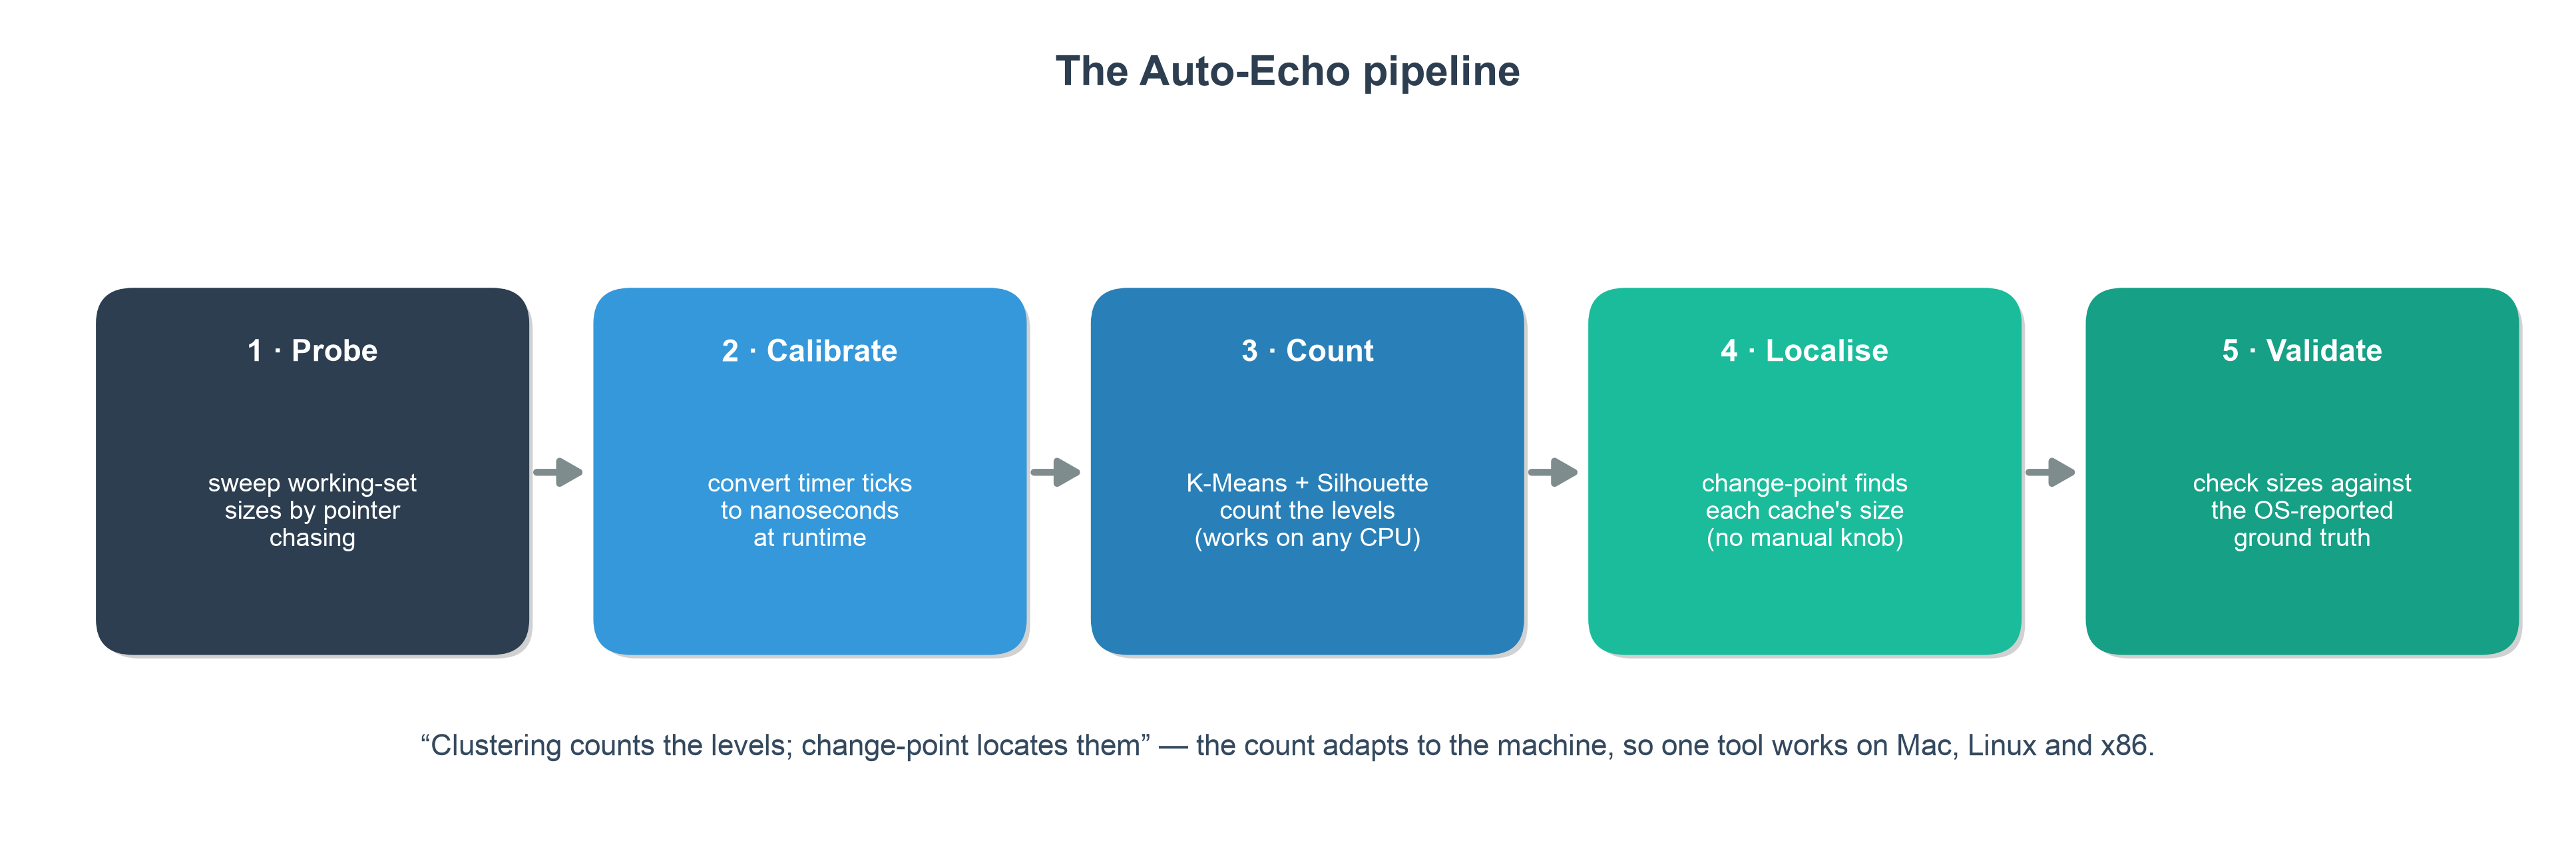
\includegraphics[width=\linewidth]{diagram_pipeline.png}}
\caption{The Auto-Echo pipeline. The probe emits a latency curve; clustering
counts the levels; change-point detection localises each boundary; validation
scores the result against operating-system ground truth. No stage receives the
number of levels as input (Fig. 1).}
\label{fig:pipeline}
\end{figure}

\subsection{A Structural Failure, and What It Constrains}

The first implementation followed the reference technique directly: flush a cache
line, write it, then time the subsequent read. It failed on both architectures,
and the reason was not the one initially assumed. Suspecting that ARM's missing
user-space flush was to blame, the same baseline was run on x86 \emph{with} a
working \texttt{clflush} and \texttt{rdtscp}. It failed there too, resolving two
tiers on a four-level machine and reporting a mean ``L1'' latency of 178\,ns
--- two orders of magnitude above that core's true 1.6\,ns L1.

The fault was structural rather than architectural. \textbf{Writing a line
immediately before timing its read pulls that line into L1, so every measurement
is an L1 hit by construction}; the flush accomplishes nothing because the store
simply re-populates the line. A per-architecture port would not have helped. The
measurement design itself had to satisfy three constraints simultaneously: never
write before reading, never time a single access, and never require a flush
primitive. Every subsequent design decision follows from one of the three.

\subsection{The Working-Set-Size Pointer-Chase Probe}

The probe measures load-to-use latency as a function of working-set size $S$.
For each $S$, a page-aligned buffer is divided into slots one cache line apart,
the line size being detected at run time (128\,B on Apple Silicon, 64\,B on
x86). The slots are then linked into a \textbf{single random Hamiltonian cycle}
by a Fisher--Yates shuffle \citep{knuth1997} driven by a seeded
\texttt{xorshift64} generator, so
every sweep is reproducible from its seed. Constructing the cycle writes every
slot, which pre-faults every page before timing begins.

Traversal is a data-dependent \textbf{pointer chase}: each load returns the
address of the next. Three properties follow, and together they discharge all
three constraints above.

\textbf{The prefetcher is defeated without a flush.} Addresses are unpredictable,
so stride and stream engines cannot run ahead. A working set larger than a given
cache overflows it \emph{by construction}, which removes the need for any explicit
eviction instruction --- essential on macOS/ARM64, where none is available to user
space.

\textbf{Memory-level parallelism is pinned to one.} The address of load $n{+}1$ is
the \emph{result} of load $n$, so the out-of-order engine cannot issue them
concurrently. This is what makes the measurement a latency rather than a
bandwidth: independent loads would overlap across the miss-handling registers and
report roughly the true latency divided by the achieved parallelism.

\textbf{No hardware fence is required.} Because the chase is already fully
serialised by data dependency, there is nothing for a memory fence to order. The
implementation uses only a \emph{compiler} barrier around the timed region ---
empty inline assembly with a memory clobber, which emits no instruction and costs
no cycles. A fence inside the loop would add real cycles to every hop, inside the
window being measured. On x86 the timestamp is read with \texttt{rdtscp} rather
than \texttt{rdtsc}, so prior instructions retire before the counter is sampled;
on ARM64 an \texttt{isb} precedes the \texttt{cntvct\_el0} read, which is an
instruction-synchronisation barrier guarding the counter read, not a memory fence
guarding the loads.

A single detail deserves emphasis because getting it wrong is silent. The value
that keeps the chase alive is stored to a \texttt{void~*volatile} sink --- a
\emph{volatile pointer}, not a pointer to volatile. The volatile store is an
observable side effect the compiler must emit, and emitting it requires the whole
dependent chain. Declared the other way round the store is dead, and
\texttt{-O3} removes the entire timed loop, reporting physically impossible
latencies near zero rather than failing.

\subsubsection{Batch-Amortised Timing}

Apple Silicon's counter advances at 24\,MHz --- roughly 41.7\,ns per tick, from a
\texttt{mach\_timebase\_info} rational of $125/3$ --- against an L1 hit of about
1.53\,ns. The timer is \emph{27 times coarser than the signal}, so timing one
access yields zero or one tick and nothing between.

The probe therefore never times a single access. It times $N \geq 2^{20}$
dependent hops in one window and divides by $N$. At 1.53\,ns per hop the window
spans ${\sim}1.6$\,ms, or ${\sim}38{,}500$ ticks, so a $\pm 1$-tick quantisation
is $\pm 0.0026\%$ of the total; and because $N$ is an exact integer chosen by the
program, dividing by it introduces no further uncertainty. The requirement this
imposes is \emph{stationarity}: per-hop cost must not drift within the window.
Three mechanisms protect it. A warm-up traversal precedes timing, so cold misses
and TLB fill do not fall inside the window. Each size is measured $R=5$ times and
the \textbf{minimum} retained, following lmbench practice \citep{mcvoy1996} on the
argument that interference can only add time. And the sweep visits sizes in \textbf{seed-shuffled order} rather than
ascending, which matters more than it appears: in ascending order the die warms
monotonically with working-set size, so thermal drift would masquerade as a
latency increase correlated with size --- precisely the shape of a real cache
boundary, and reproducible enough to survive a repeat run. Shuffling converts that
systematic bias into noise.

\subsubsection{Runtime Timer Calibration}

Converting ticks to nanoseconds is itself a portability problem. The reference
implementation parses the \texttt{cpu MHz} field of \texttt{/proc/cpuinfo}, which
is Linux-only and, more seriously, reports the \emph{current turbo-scaled core
clock} while \texttt{rdtsc} advances at the fixed invariant-TSC rate. Auto-Echo
instead \textbf{calibrates at run time}, counting hardware ticks over a 50\,ms
interval of the OS monotonic clock (\texttt{clock\_gettime}, or
\texttt{QueryPerformanceCounter} on Windows).

The Intel machine supplies a quantitative reason this matters. Windows advertises
the part at 2.40\,GHz; calibration measures 0.383\,ns/tick, a 2.61\,GHz invariant
TSC --- a discrepancy of 8.8\%. Both figures are correct, because they describe
different clocks: 2.40\,GHz is the performance-core base frequency, whereas the
invariant TSC ticks at a reference rate deliberately decoupled from it. Had the
framework taken the advertised value, every reported latency would be inflated by
8.8\% while every detected \emph{capacity} --- a working-set size, which never
passes through the tick conversion --- remained correct. The error would have been
confined to the one column no internal consistency check could expose.

\subsection{Level Discovery: Count, then Localise}

A cache of capacity $C$ holds latency flat while $S \leq C$ and steps up once it
overflows, so the number of memory levels is the number of \emph{plateaus} in the
latency-versus-$\log S$ curve, and each capacity is the size at the
plateau-to-rise transition. Turning that observation into an algorithm runs
immediately into a difficulty: both the clustering objective and the segmentation
objective are monotonically non-increasing in the number of components, so
neither can select its own. Minimising either returns the degenerate answer in
which every observation is its own level.

Auto-Echo resolves this by splitting the problem between two stages that use
different information, and giving each only the statistic sufficient for its own
question.

\textbf{Counting is order-ignoring.} ``How many latency regimes exist?'' is a
question about the \emph{distribution} of latency values, not their arrangement,
so the stage operates on the multiset of per-size log-latencies. The count is
chosen by the \textbf{silhouette coefficient} \citep{rousseeuw1987}, which unlike inertia is not
monotone in $k$: it scores cohesion against separation, and splitting a genuine
plateau places two near-identical clusters adjacent to one another, collapsing the
separation term. It therefore has an interior maximum and needs no penalty
parameter.

The partition itself is solved \emph{exactly}. On the real line an optimal
$k$-means partition is necessarily contiguous in sorted order, which reduces the
search from a Stirling number of set partitions to a choice of $k-1$ cut points
and admits an exact dynamic program in $O(kn^2)$ \citep{fisher1958,wang2011}
(Appendix~\ref{app:dp}). Prefix
sums of $x$ and $x^2$ make each candidate segment's cost $O(1)$. Using the exact
solver in place of Lloyd's heuristic \citep{lloyd1982} buys no accuracy on the measured curves ---
both reach the same $k$ --- but it makes optimality a property of the algorithm
rather than an observation about two data sets, and it removes seeding, restarts
and random state, so repeated runs are bit-identical. That matters because the
evaluation reports variability across sweeps, and solver-induced variance would
contaminate a hardware measurement.

\textbf{Localisation is order-respecting.} ``Where does each level end?'' is a
question about position along the size axis, so the second stage segments the
ordered curve. Crucially it is given the count from the first stage and asked for
exactly $k-1$ breakpoints, using a \emph{count-constrained} dynamic program \citep{truong2020}. This
is what keeps the pipeline free of thresholds: a penalty-based segmenter such as
PELT \citep{killick2012} would require choosing a penalty, and that penalty --- not the data ---
would determine how many levels were reported. PELT is used in this work only as
a sensitivity instrument, sweeping the penalty to confirm that the recovered count
is not balanced on a knife-edge.

Segmentation operates on \textbf{log}-latency. Under a squared-error cost on raw
nanoseconds the deepest transition dominates: on the M1 the L2$\rightarrow$DRAM
step is worth roughly 250 times more cost reduction than L1$\rightarrow$L2, so a
segmenter with a limited budget of breakpoints would spend them subdividing the
DRAM region and never place the L1 boundary at all. Caches are laid out
multiplicatively, so the physically meaningful quantity is a ratio; taking
logarithms makes a factor-of-six step cost the same whether it occurs at 1.5\,ns
or at 130\,ns.

Because the two stages consume different information, their agreement is
informative rather than circular, and three further estimators --- the elbow
criterion, a Gaussian mixture and DBSCAN, all via scikit-learn
\citep{pedregosa2011} --- are run alongside as independent cross-checks. None of them feeds the productive path.

\subsection{Validation}

Detected boundaries are matched to operating-system ground truth by optimal
one-to-one (Hungarian) assignment, with a match declared when the capacities agree
within a factor of two, i.e. one octave. Ground truth is read \emph{per core}
rather than per socket, which is essential on heterogeneous parts: the generic
macOS keys report the efficiency cluster, and scoring a performance-core
measurement against them would compare a Firestorm result to Icestorm hardware.
Capacities are reported as the \textbf{median of per-sweep detections} rather
than detected once on the aggregated curve, for a reason quantified in
Section~\ref{sec:eval}.

%% ===========================================================================
\section{Results and Evaluation}
\label{sec:eval}
%% TARGET 3200 words / 4.7 pages + Figs 2-3 + Tables I-III

\subsection{Machines and Ground Truth}

Two machines were measured: an \textbf{Apple M1} (ARM64, Firestorm performance
core, 128\,B line, 16\,KiB base page) running macOS, and an \textbf{Intel Core
i5-13450HX} (x86-64, Raptor Lake performance core, 64\,B line, 4\,KiB base page)
running Windows. Both are consumer laptop parts, which bounds the generalisation
claim and is returned to in Section~\ref{sec:discussion}.
Table~\ref{tab:lenses} sets out what each of the three lenses of
Section~\ref{sec:intro} reports for each machine.

\begin{table}[t]
\caption{The two machines under all three lenses. The vendor report names no
cache on either machine; \texttt{lstopo} is complete on the Intel part and silent
about the M1's System-Level Cache; only measurement responds to it.}
\label{tab:lenses}
\centering
\footnotesize
\begin{tabular}{@{}lll@{}}
\toprule
& \textbf{Apple M1} & \textbf{Intel i5-13450HX} \\
\midrule
ISA, core            & ARM64, Firestorm   & x86-64, Raptor Lake \\
Line, base page      & 128\,B, 16\,KiB    & 64\,B, 4\,KiB \\
\midrule
\multicolumn{3}{@{}l}{\emph{Lens 1 --- vendor system report}} \\
\quad Cache data     & \textbf{none}      & \textbf{none} \\
\midrule
\multicolumn{3}{@{}l}{\emph{Lens 2 --- \texttt{lstopo} / OS descriptors}} \\
\quad L1d            & 128\,KB            & 48\,KB \\
\quad L2             & 12\,MB (cluster)   & 1280\,KB per core \\
\quad Last level     & \textbf{not reported} & 20\,MB shared \\
\midrule
\multicolumn{3}{@{}l}{\emph{Lens 3 --- Auto-Echo}} \\
\quad Levels found   & 3                  & 4 (2\,MiB pages) \\
\quad Deepest band   & 13.9\,MiB          & 19.7\,MiB \\
\bottomrule
\end{tabular}
\end{table}

Ground truth is read \emph{per core}. On macOS this means
\texttt{hw.perflevel0.*} rather than the generic \texttt{hw.*} keys, and the
distinction is not cosmetic: the generic keys report the \emph{efficiency}
cluster, so scoring the performance-core probe against them would compare a
Firestorm measurement to Icestorm hardware and inflate the L1 error from
$+23.0\%$ to $+146\%$ --- outside the matching tolerance, turning a correct
result into a reported failure. On Windows the equivalent is
\texttt{GetLogicalProcessorInformationEx} filtered to the caches serving CPU 0,
rather than the per-socket \texttt{Win32\_CacheMemory} aggregate.

Because the evaluation scores the probe \emph{against} this ground truth, the
ground truth is itself a reference standard and needs verifying rather than
assuming. It was therefore cross-checked against \texttt{hwloc}
\citep{broquedis2010}, an independent implementation, on every machine. Two
points follow. Where the operating system reports a cache, \texttt{hwloc} agrees
with the framework's own reader on every value, so the reference standard is
verified. But \texttt{hwloc} reads the same interfaces, so where the OS is silent
it is silent too: it is an independent \emph{implementation}, not an independent
\emph{source}. The M1's System-Level Cache is missing from \texttt{lstopo}
exactly as it is missing from \texttt{sysctl}.

\subsection{Discovered Hierarchies}

Fig.~\ref{fig:mountain} shows the recovered latency curves. The pipeline received
no hint of how many levels either machine has.

\begin{figure}[t]
\centerline{
\includegraphics[width=\linewidth]{compare_mountain.png}}
\caption{Latency against working-set size for both machines on one log--log
axis, with each machine's automatically detected boundaries marked. The Intel
curve is the 2\,MiB huge-page run; under the default 4\,KiB pages its L3 step is
absent entirely (Table~\ref{tab:pagesize}).}
\label{fig:mountain}
\end{figure}

On the \textbf{Apple M1} all five estimators agree on \textbf{three} levels. The
L1 plateau sits at 1.53\,ns and ends at a detected 157.5\,KiB; a middle band at
9.19\,ns extends to 13.9\,MiB; DRAM follows at 130.43\,ns. The middle band is the
interesting one, because the operating system documents a 12\,MiB L2 and nothing
beyond it. The probe responds to capacity roughly 16\% past that figure, and the
only structure that can supply the difference is the ${\sim}8$\,MiB System-Level
Cache that no interface reports. The L2 and the SLC are not separated: they
resolve as a single band, and no estimator splits them. That is an honest limit
of a one-dimensional latency sweep --- two adjacent tiers with similar latency
merge --- and it is reported as one band rather than presented as two.

On the \textbf{Intel} part, under a 2\,MiB huge-page allocation, the same
unsupervised code path recovers \textbf{four} levels: L1 at 1.57\,ns to
55.7\,KiB, L2 at 4.71\,ns to 1.2\,MiB, L3 at 20.81\,ns to 19.7\,MiB, and DRAM at
122.36\,ns. This is the framework's first full L1/L2/L3/DRAM recovery, and it is
reported with its provenance: it is a property of the huge-page run, not of
default behaviour.

The two machines exercise the same code path on different ISAs, different line
sizes (128\,B against 64\,B) and different page sizes (16\,KiB against 4\,KiB),
with no per-machine configuration and no supplied level count. That is the
substance of the architecture-agnostic claim.

\subsection{Consolidated Validation}

Table~\ref{tab:validation} places every documented cache on both machines against
both reference sources: what the operating system says, what an independent
implementation says, what Auto-Echo measured, and whether they agree.

\begin{table}[t]
\caption{Consolidated validation. Ground truth as read per core; \texttt{hwloc}
as an independent cross-check; detected capacities as the median of per-sweep
detections. A match requires agreement within a factor of two, i.e. an absolute
error of at most one octave. Intel figures are the 2\,MiB huge-page run.}
\label{tab:validation}
\centering
\footnotesize
\begin{tabular}{@{}llrrrc@{}}
\toprule
\textbf{Machine} & \textbf{Cache} & \textbf{OS} & \textbf{Detected} &
\textbf{Error} & \textbf{Match} \\
\midrule
Apple M1 & L1d  & 128\,KiB   & 157.5\,KiB & $+23.0\%$ & \cmark \\
Apple M1 & L2   & 12\,MiB    & 13.9\,MiB  & $+16.1\%$ & \cmark \\
Apple M1 & SLC  & \emph{n/r} & \emph{--}  & \emph{--} & \emph{n/s} \\
Intel i5 & L1d  & 48\,KiB    & 55.7\,KiB  & $+16.0\%$ & \cmark \\
Intel i5 & L2   & 1.25\,MiB  & 1.2\,MiB   & $-1.5\%$  & \cmark \\
Intel i5 & L3   & 20\,MiB    & 19.7\,MiB  & $-1.5\%$  & \cmark \\
\bottomrule
\end{tabular}
\\[2pt]
\raggedright\footnotesize
\emph{n/r} = not reported by any OS interface; \emph{n/s} = not scorable, because
no ground truth exists to score against. \texttt{hwloc} agrees with the OS on
every row except SLC, where both are silent.
\end{table}

\textbf{Five documented caches, five matches, on two architectures.} Recall is
2/2 on the M1 and 3/3 on the Intel part, at 100\% precision on both: no detected
knee is a false positive. Errors span $-1.5\%$ to $+23.0\%$, and the two x86
inner levels land within 0.02 octaves of nominal.

Three points about this table deserve stating, because each answers a question a
reader should be asking.

First, \textbf{the errors are one-signed on private caches, and that is a
property of the estimator rather than noise}. Because the chase visits the
working set in random order, a set moderately larger than the cache still enjoys
high residency --- at 157.5\,KiB against a 128\,KiB L1, roughly 81\% of accesses
still hit --- so average latency rises gently past nominal rather than stepping.
The detected plateau therefore extends slightly beyond true capacity, and it does
so \emph{upward} every time. The diagnosis is testable: an alternative
\emph{onset} estimator, which fires at the first departure from the plateau
median, recovers the M1 L1 at exactly 128\,KiB ($+0.0\%$). It is not adopted as
the default because it is unreliable elsewhere, under-reading three of the other
four levels by 71--97\% (Appendix~\ref{app:robustness}). This is an explicit
accuracy-versus-robustness trade, decided for robustness.

Second, \textbf{the SLC row is deliberately unscorable rather than omitted}. No
ground truth exists for it, so no error can be computed and reporting one would
be fabrication. It is nevertheless the row that most justifies the method: the
probe reaches 13.9\,MiB against a documented 12\,MiB L2, and only the unreported
tier can account for the difference.

Third, \textbf{a match is a claim about an octave, not a percentage.} The
defensible statement is that every documented cache has a detected boundary
within a factor of two of its nominal capacity, and on that statement the
framework is 5/5.

\subsection{Page Size Decides Whether a Cache Is Visible}

The Intel result above is conditional, and the condition is the sharpest finding
in this work. Under the machine's \emph{default} 4\,KiB pages, the documented
20\,MiB L3 is not merely harder to detect --- it is behaviourally unreachable.

\begin{table}[t]
\caption{The same Intel silicon under two page sizes. Nothing about the cache
hierarchy differs between columns; only the translation path does.}
\label{tab:pagesize}
\centering
\footnotesize
\begin{tabular}{@{}lcc@{}}
\toprule
& \textbf{4\,KiB pages} & \textbf{2\,MiB huge pages} \\
\midrule
L3 boundary reported   & ${\sim}3.5$\,MiB & \textbf{19.7\,MiB} \\
Deep-plateau latency   & ${\sim}143$\,ns  & \textbf{20.81\,ns} \\
Caches matched         & 2/3              & \textbf{3/3} \\
Level count, per sweep & unstable (2--5)  & \textbf{4 (std 0.00)} \\
Silhouette at selected $k$ & 0.885        & \textbf{0.933} \\
\bottomrule
\end{tabular}
\end{table}

The mechanism is TLB reach. A first-level data TLB of ${\sim}96$ entries spans
${\sim}384$\,KiB under 4\,KiB pages and ${\sim}192$\,MiB under 2\,MiB pages ---
a factor of 512, exactly the page-size ratio. A 20\,MiB working set therefore
spans 5{,}120 pages against 96 entries, a 53-fold over-subscription. Long before
the working set approaches L3 capacity, every dependent load misses in the TLB
and triggers a page-table walk whose own accesses miss to DRAM. Past
${\sim}1.3$\,MiB the curve climbs steeply and \emph{saturates} at a flat
${\sim}143$\,ns plateau by 4--5\,MiB, staying there to 64\,MiB. A saturated curve
has no knee, so there is nothing for the inference stage to localise.

Four independent lines of evidence establish that the ${\sim}3.5$\,MiB band the
segmenter reports under 4\,KiB pages is a TLB-transition artefact and not a
cache. Its plateau latency is ${\sim}143$\,ns, seven times this part's true L3
hit and essentially equal to DRAM --- a structure that is not faster than what it
fronts is not a cache. Its position is wrong by a factor of 5.7 against the
documented 20\,MiB, so the validation layer scores it as a miss. The curve never
leaves that plateau out to 64\,MiB, whereas a genuine 3.5\,MiB cache would be
followed by a further step into DRAM. And, decisively, changing \emph{one}
variable removes it: under 2\,MiB pages the artefact disappears and a feature
matching the documented L3 to $-1.5\%$ appears in its place. The artefact was
falsified by intervention, not inferred from its shape.

The wider consequence is the one drawn in Section~\ref{sec:intro}. Here the
topology descriptor is entirely correct --- there is a 20\,MiB L3 --- and the
answer it gives is still not the answer a performance engineer needs, because
reachability depends on the page size the allocation happens to use. No entry a
topology tool could add would fix that, since the property being asked about
belongs to the running system rather than to the die.

\subsection{Contention Sets the Mappable Share of a Shared Cache}

A second boundary condition concerns sharing. The Intel L3 is shared across all
cores over a ring interconnect, so what a single probing core recovers is not the
cache's capacity but the share left to it. Fig.~\ref{fig:contention} shows the
effect measured directly, with eight worker threads streaming 32\,MiB buffers on
other physical cores while the probe runs.

\begin{figure}[t]
\centerline{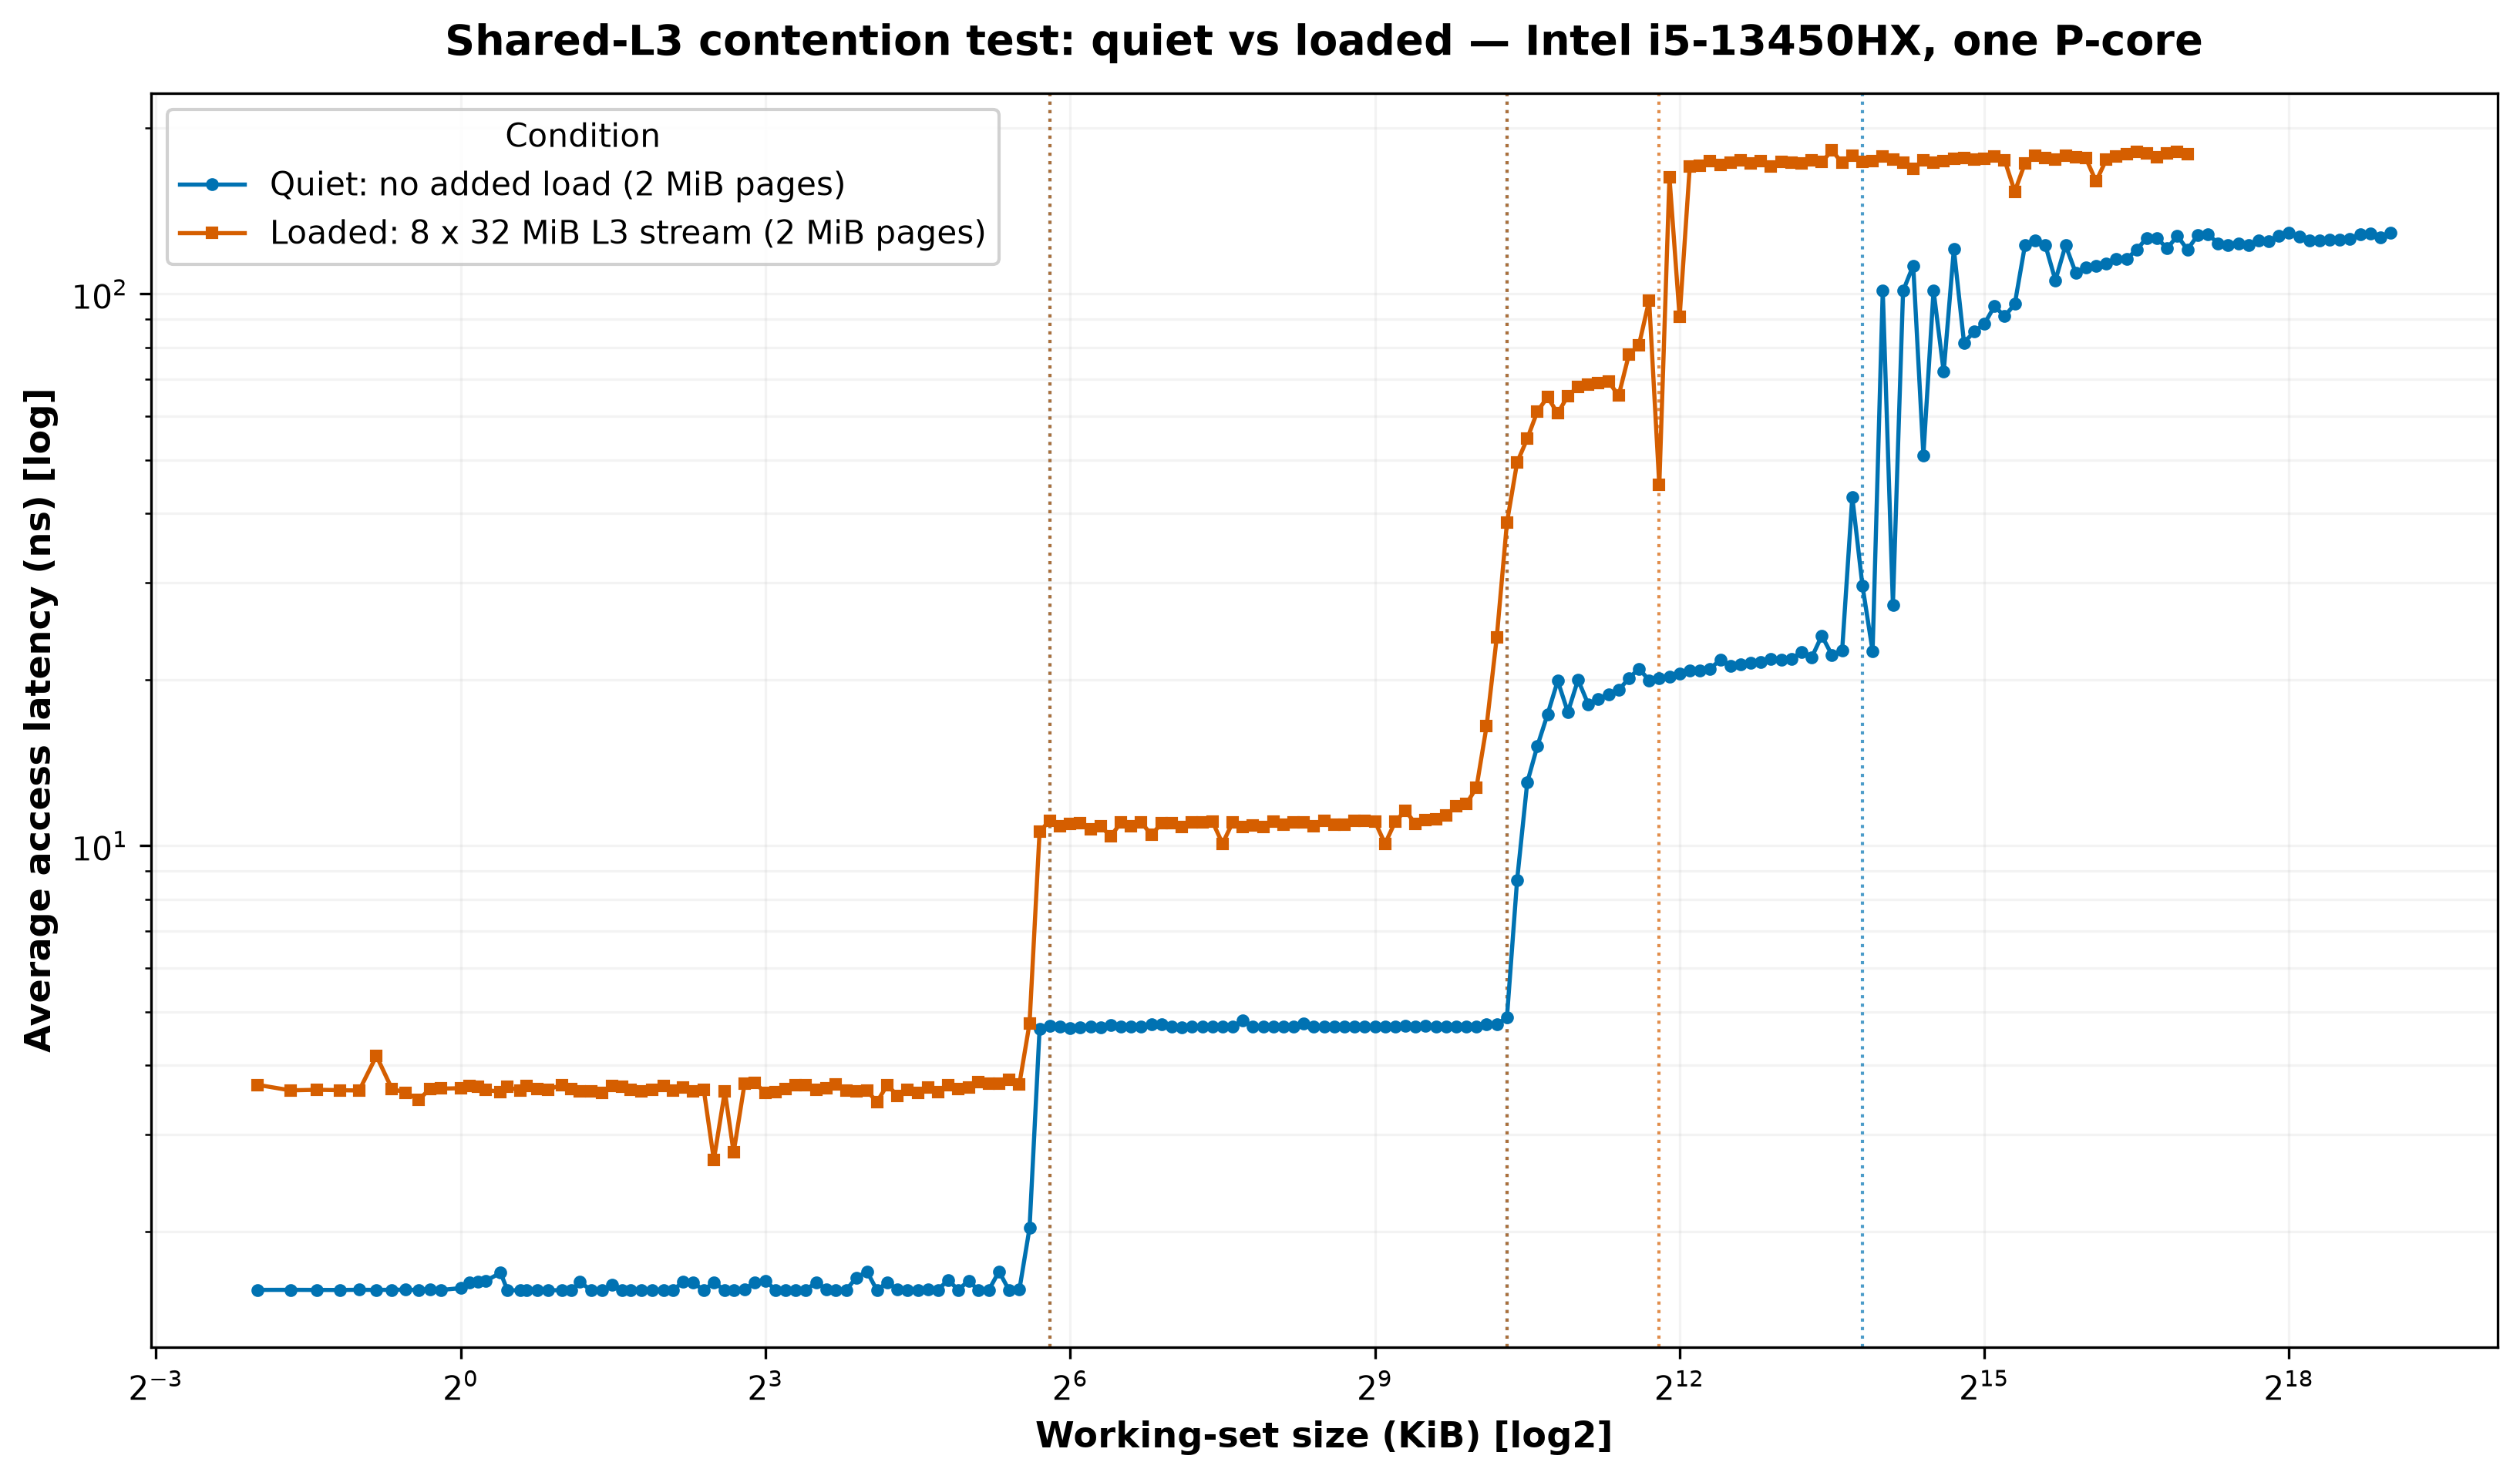
\includegraphics[width=\linewidth]{l3_contention_intel.png}}
\caption{The Intel L3 under load. Eight streaming workers on other physical
cores drive the detected L3 boundary from 19.7\,MiB to 3.5\,MiB --- a factor of
5.6 --- with zero within-condition spread.}
\label{fig:contention}
\end{figure}

The detected L3 collapses from \textbf{19.7\,MiB} ($-1.5\%$ of nominal) to a
stable \textbf{3.5\,MiB} ($-83\%$) in every loaded sweep. The private L1 and L2
capacities are unchanged, exactly as expected: no other core can allocate into
them, and the workers were pinned so that the probe's own physical core stayed
idle, excluding SMT interference within it.

Every latency also rises by a uniform factor of ${\sim}2.2$ under load, and it
would be easy to mistake that for the cause of the capacity change. It is not,
and the two effects are separable by observation. The multiplier is already
present at a \textbf{256\,B} working set, where the shared L3 cannot be
implicated at all; a uniform, size-independent scaling is the signature of a
\emph{clock} effect rather than a cache effect. More importantly, the two act on
different axes: a multiplier on latency rescales the curve vertically and cannot
move the working-set size at which a plateau ends. The knee is a size, and sizes
are frequency-invariant.

The clock effect is attributed to the loss of single-core turbo, but its
magnitude is \emph{not} claimed to be accounted for: this part's 4.6\,GHz
single-core turbo against a 2.4\,GHz base spans only ${\sim}1.9\times$, so a
$2.2\times$ rise implies operation below base frequency, an additional uncore
component, or both. The framework cannot settle it, because the runtime
calibration measures the \emph{invariant} TSC, whose rate is by construction
decoupled from the core clock --- the same property that makes it a trustworthy
timebase makes it useless as a tachometer. Resolving this needs
\texttt{APERF}/\texttt{MPERF} or an OS performance counter, both privileged.

\subsection{Robustness, and an External Check}

Three further results bound the confidence in the above; each is summarised here
and detailed in the appendices.

\textbf{The level count does not depend on sampling resolution.} Because the
silhouette weights every observation equally, and the number of observations per
level is fixed by the sweep grid rather than by the hardware, the selected count
could in principle be an artefact of the experimenter's chosen resolution. Re-run
end to end at 5, 10 and 20 points per octave, the count is invariant on both
machines --- 3 on the M1 and 4 on the Intel part across a four-fold density
change (Appendix~\ref{app:robustness}).

\textbf{The inference layer transfers to a curve it did not produce.} Applied
unmodified to a latency curve measured by lmbench's \texttt{lat\_mem\_rd}
\citep{mcvoy1996} on the same silicon, the pipeline selects the correct level
count and recovers both TLB-unmasked capacities (Appendix~\ref{app:lmbench}).
This tests the contribution --- the inference stage --- against prior art rather
than only against itself.

\textbf{Count stability is a property of a quiet machine, not of the part.} On a
contaminated run the productive counter over-counts, returning a modal seven
levels with a standard deviation of 1.25 and ranking last of the five estimators,
against a mean of 4.00 and standard deviation of 0.00 on the quiet ten-sweep run.
This is a genuine limitation of the counter and is carried into
Section~\ref{sec:discussion} rather than left in the repository.

\subsection{Data Availability}

The latency curves underlying the M1 results, the Intel huge-page results, and
the contention experiment are committed to the project repository as
\texttt{wss\_curve.csv} and \texttt{wss\_curves\_all.csv}, and every figure and
table above derived from them is reproducible from that data. The 4\,KiB-page
Intel run of Table~\ref{tab:pagesize} is an exception: the machine was borrowed
and is no longer available, and while the run's outputs were recorded its raw
curve was not retained. Those figures are therefore reported as measured but are
not independently re-derivable from the repository, and they are flagged as such
rather than presented on the same footing as the rest.

%% ===========================================================================
\section{Discussion}
\label{sec:discussion}
%% TARGET 1000 words / 1.2 pages

The results support a narrower claim than ``a tool that maps any cache
hierarchy'', and the difference matters. What has been demonstrated is that an
unsupervised pipeline, given no descriptor and no privileges, recovers every
documented cache on two machines of different ISAs to within one octave, and
responds to one undocumented cache that no interface reports. The boundaries on
that claim are as much a result as the claim itself.

\textbf{The evidence base is narrow.} Two machines, both consumer laptop
performance cores, is a thin foundation for a generalisation about architectures.
The recovery is genuinely cross-ISA --- 128\,B and 64\,B lines, 16\,KiB and
4\,KiB pages, ARM64 and x86-64, one code path --- but a server part, a
different-vendor core, or an efficiency core would each test the claim in a
direction these two do not. The level \emph{count} is also less unanimous than the
headline suggests: the productive counter is stable and correct on both machines,
but cross-estimator unanimity holds only on the M1, where all five agree on three
levels. On the Intel part the elbow and cost-knee criteria return two against an
expected four, and only the silhouette-based counter is right.

\textbf{The two machines are not like-for-like.} The M1 runs on a 16\,KiB base
page and the Intel on 4\,KiB, so for any given working set the M1 places a
quarter of the Intel's demand on address translation. Because the large-page path
is available only on Windows, the M1 has never been measured at any other page
size --- macOS on ARM64 rejects both \texttt{VM\_FLAGS\_SUPERPAGE\_SIZE\_2MB} and
its permissive variant with \texttt{EINVAL}, superpages being an Intel-era
facility the architecture does not honour. The cleaner deep region of the M1
curve therefore \emph{cannot} be attributed to the architecture alone; part of it
may simply be the larger page. This does not affect either machine's validation
against its own ground truth, which is what Section~\ref{sec:eval} reports, but it
forecloses the cross-machine comparison that would otherwise be tempting. The
asymmetry is not an implementation gap that more effort would close: it is a
difference in what the two platforms permit an unprivileged tool to do, which is
the same class of obstacle that motivated the design.

\textbf{Detected capacities carry a systematic bias, and its sign depends on
sharing.} For a private cache the bias is one-signed upward, for the residency
reason given in Section~\ref{sec:eval}. For a \emph{shared} cache a second,
opposing bias applies: a single probing core can only map the share left to it,
so contention pulls the estimate down. On a quiet machine these partly cancel ---
part of why the Intel L3 reads a flattering $-1.5\%$ --- and under load the
downward term dominates completely, reaching $-83\%$. A number whose sign depends
on the ambient load of the rest of the system is not a constant of the hardware,
which is why the L3 result is reported with its load condition attached.

\textbf{No inferential statistics are claimed.} Level counts are reported with a
standard deviation and capacities with a non-parametric min--max spread across
sweeps; no hypothesis test is performed and no confidence interval is quoted. Ten
sweeps is too few for a parametric interval, and reporting a standard error as
though it were one would overstate what the data supports. Where a comparison is
made --- quiet against loaded --- it rests on a five-fold effect with zero
within-condition spread, not on a significance claim.

\textbf{What is measured is load-to-use latency of a serialised chain}, which
includes base pipeline cost. Absolute values are therefore best read as relative
differences between tiers rather than as architectural constants comparable
across measurement methodologies.

\textbf{Two threats are acknowledged rather than resolved.} On Apple Silicon the
probe relies on randomisation defeating the prefetcher, yet
\citet{vicarte2022} demonstrated a data memory-dependent prefetcher on that exact
part which follows pointer-like values --- precisely the pattern this probe
generates. The measured curves show clean, well-separated plateaus and a DRAM
plateau at 130\,ns consistent with unprefetched access, so the effect is not large
enough here to flatten the staircase; but that is an empirical observation on one
part, not a guarantee. Second, macOS exposes no user-space CPU-affinity API, so
the probe requests a performance-cluster quality-of-service class rather than
pinning. Calling that ``pinning'' would overstate it. Two checks show the bias
took effect: \texttt{hwloc} confirms the clusters differ in cache geometry, and
the recovered capacities score $+23.0\%$ and $+16.1\%$ against performance-core
figures where the same measurements would read $+146\%$ and $+248\%$ against the
efficiency cluster --- far outside tolerance, so the result could not have come
from the wrong cores.

%% ===========================================================================
\section{Conclusion and Future Work}
\label{sec:conclusion}
%% TARGET 650 words / 0.8 pages

This paper asked whether a program can discover its machine's cache hierarchy for
itself, from timing alone, with no privileges, no vendor tables and no
architecture-specific instructions. On two machines it can. A flush-free
pointer-chase probe with batch-amortised, runtime-calibrated timing feeds an
unsupervised stage in which exact one-dimensional clustering counts the memory
levels and count-constrained change-point detection localises each capacity, with
no threshold, no penalty and no supplied level count anywhere in the productive
path. Every documented cache on both machines was recovered and matched within a
factor of two: 2/2 on the Apple M1 and 3/3 on the Intel part, at 100\% precision,
against ground truth independently cross-checked with \texttt{hwloc}.

The three lenses of Section~\ref{sec:intro} are, in the end, the clearest
statement of what this contributes. The commercial lens names no cache on either
machine. The software lens is accurate wherever a vendor filled in the table ---
and on the Intel part it is entirely accurate, which this paper asserts rather
than disputes; any argument for measurement resting on \texttt{lstopo} being
\emph{wrong} would be false. Its limit is that its chain of trust ends at what the
operating system was told, so it inherits every omission, and it can only ever
describe the hardware as designed. The physical lens answers a different question
--- what this silicon does, on this run, at this page size, under this load ---
and the two machines show that the gap between those questions is not a
technicality. On the M1 the gap is an entire ${\sim}8$\,MiB cache that no
interface reports. On the Intel part it is a 20\,MiB L3 that is documented,
correct, and unreachable. Neither gap is visible to a table, and neither is
discoverable by asking more politely. The case is for \emph{complementing} the
first two lenses, not replacing them.

Three extensions follow directly.

\textbf{An AMD Zen part is the highest-value next measurement}, because it
differs from the Intel machine in precisely the variable the contention
experiment isolates. Raptor Lake's L3 is a single last-level cache shared over a
ring interconnect, which is why eight streaming workers drove the recovered
capacity down five-fold. Zen's L3 is instead a victim cache private to each core
complex, with inter-complex traffic crossing a separate fabric. The prediction is
specific and falsifiable: workers pinned to the probe's \emph{own} complex should
reproduce the under-read, while workers on a \emph{different} complex should leave
its slice largely intact, since they do not compete for the same physical cache.
Confirming this would establish that the experiment measures cache \emph{sharing}
rather than system load; failing to confirm it would bound the finding to
ring-based last-level caches. Either outcome is a result.

\textbf{A page-size control on Apple Silicon} would resolve the confound of
Section~\ref{sec:discussion}, but is blocked by the platform rather than by
effort. It would require either a privileged allocation path or an unprivileged
large-page interface that macOS on ARM64 does not currently provide.

\textbf{Direct instrumentation of the two effects this work can only infer.}
Performance counters exposing DTLB-miss and page-walk-cycle events would confirm
the translation mechanism of Table~\ref{tab:pagesize} independently of the
page-size manipulation, and the \texttt{APERF}/\texttt{MPERF} pair would settle
whether the uniform $2.2\times$ slowdown under load is entirely a core-frequency
effect. Both are privileged, so both sit outside this project's constraint ---
which is itself the point: the boundary of what unprivileged measurement can
establish is exactly where those instruments become necessary.

%% ===========================================================================
%% References and appendices do NOT count against the 12-page limit (Sec. 4.3.1)
%%
%% Harvard format per Guide Sec. 8.2. Note the house style precisely:
%%   - no comma between author and year in text: (Leyden 2005)
%%   - "et al" with NO full stop
%%   - journal: Author, A.B. (Year). Title. Journal, vol (issue), pages.
%%   - web:     Author, A. (Year) Title. Site [on-line]. Available from URL
%%              [Accessed D Month YYYY]
%% ===========================================================================
\begin{thebibliography}{99}

\bibitem[Broquedis et al(2010)]{broquedis2010}
Broquedis, F., Clet-Ortega, J., Moreaud, S., Furmento, N., Goglin, B.,
Mercier, G., Thibault, S. \& Namyst, R. (2010). hwloc: a generic framework for
managing hardware affinities in HPC applications. \textit{Proceedings of the 18th
Euromicro International Conference on Parallel, Distributed and Network-Based
Processing}, 180--186.

\bibitem[Bryant and O'Hallaron(2015)]{bryant2015}
Bryant, R.E. \& O'Hallaron, D.R. (2015). \textit{Computer Systems: A
Programmer's Perspective}. 3rd ed. Boston: Pearson.

\bibitem[Chen et al(2024)]{chen2024}
Chen, B., Wang, Y., Shome, P., Fletcher, C.W., Kohlbrenner, D., Paccagnella, R.
\& Genkin, D. (2024). GoFetch: breaking constant-time cryptographic
implementations using data memory-dependent prefetchers. \textit{Proceedings of
the 33rd USENIX Security Symposium}, 1117--1134.

\bibitem[Drepper(2007)]{drepper2007}
Drepper, U. (2007) What every programmer should know about memory. \textit{LWN.net}
[on-line]. Available from \url{https://lwn.net/Articles/250967/} [Accessed 4 August 2026].

\bibitem[Fisher(1958)]{fisher1958}
Fisher, W.D. (1958). On grouping for maximum homogeneity. \textit{Journal of the
American Statistical Association}, 53 (284), 789--798.

\bibitem[Gr\o{}nlund et al(2017)]{gronlund2017}
Gr\o{}nlund, A., Larsen, K.G., Mathiasen, A., Nielsen, J.S., Schneider, S. \&
Song, M. (2017) Fast exact $k$-means, $k$-medians and Bregman divergence
clustering in 1D. \textit{arXiv} [on-line]. Available from
\url{https://arxiv.org/abs/1701.07204} [Accessed 4 August 2026].

\bibitem[Intel(2023)]{intel2023}
Intel Corporation (2023). \textit{Intel 64 and IA-32 Architectures Software
Developer's Manual, Volume 2A: Instruction Set Reference}. Santa Clara, CA: Intel
Corporation.

\bibitem[Intel(2024)]{intel_mlc}
Intel Corporation (2024) Intel Memory Latency Checker (Intel MLC) [on-line].
Available from \url{https://www.intel.com/content/www/us/en/developer/articles/tool/intelr-memory-latency-checker.html}
[Accessed 4 August 2026].

\bibitem[Killick et al(2012)]{killick2012}
Killick, R., Fearnhead, P. \& Eckley, I.A. (2012). Optimal detection of
changepoints with a linear computational cost. \textit{Journal of the American
Statistical Association}, 107 (500), 1590--1598.

\bibitem[Knuth(1997)]{knuth1997}
Knuth, D.E. (1997). \textit{The Art of Computer Programming, Volume 2:
Seminumerical Algorithms}. 3rd ed. Reading, MA: Addison-Wesley.

\bibitem[Lloyd(1982)]{lloyd1982}
Lloyd, S.P. (1982). Least squares quantization in PCM. \textit{IEEE Transactions
on Information Theory}, 28 (2), 129--137.

\bibitem[McVoy and Staelin(1996)]{mcvoy1996}
McVoy, L. \& Staelin, C. (1996). lmbench: portable tools for performance
analysis. \textit{Proceedings of the USENIX Annual Technical Conference},
279--294.

\bibitem[Osvik et al(2006)]{osvik2006}
Osvik, D.A., Shamir, A. \& Tromer, E. (2006). Cache attacks and countermeasures:
the case of AES. \textit{Topics in Cryptology --- CT-RSA 2006}, LNCS 3860,
1--20. Berlin: Springer.

\bibitem[Percival(2005)]{percival2005}
Percival, C. (2005) Cache missing for fun and profit. \textit{Proceedings of
BSDCan 2005} [on-line]. Available from \url{https://www.daemonology.net/papers/cachemissing.pdf}
[Accessed 4 August 2026].

\bibitem[Rousseeuw(1987)]{rousseeuw1987}
Rousseeuw, P.J. (1987). Silhouettes: a graphical aid to the interpretation and
validation of cluster analysis. \textit{Journal of Computational and Applied
Mathematics}, 20, 53--65.

\bibitem[Saavedra and Smith(1995)]{saavedra1995}
Saavedra, R.H. \& Smith, A.J. (1995). Measuring cache and TLB performance and
their effect on benchmark run times. \textit{IEEE Transactions on Computers},
44 (10), 1223--1235.

\bibitem[Pedregosa et al(2011)]{pedregosa2011}
Pedregosa, F., Varoquaux, G., Gramfort, A., Michel, V., Thirion, B., Grisel, O.,
Blondel, M., Prettenhofer, P., Weiss, R., Dubourg, V., Vanderplas, J., Passos, A.,
Cournapeau, D., Brucher, M., Perrot, M. \& Duchesnay, E. (2011). Scikit-learn:
machine learning in Python. \textit{Journal of Machine Learning Research}, 12,
2825--2830.

\bibitem[Terpstra et al(2010)]{terpstra2010}
Terpstra, D., Jagode, H., You, H. \& Dongarra, J. (2010). Collecting performance
data with PAPI-C. \textit{Tools for High Performance Computing 2009}, 157--173.
Berlin: Springer.

\bibitem[Treibig et al(2010)]{treibig2010}
Treibig, J., Hager, G. \& Wellein, G. (2010). LIKWID: a lightweight
performance-oriented tool suite for x86 multicore environments.
\textit{Proceedings of the 39th International Conference on Parallel Processing
Workshops}, 207--216.

\bibitem[Truong et al(2020)]{truong2020}
Truong, C., Oudre, L. \& Vayatis, N. (2020). Selective review of offline change
point detection methods. \textit{Signal Processing}, 167, 107299.

\bibitem[Vicarte et al(2022)]{vicarte2022}
Vicarte, J.R.S., Flanders, M., Paccagnella, R., Garrett-Grossman, G., Morrison,
A., Fletcher, C.W. \& Kohlbrenner, D. (2022). Augury: using data
memory-dependent prefetchers to leak data at rest. \textit{Proceedings of the
IEEE Symposium on Security and Privacy}, 1491--1505.

\bibitem[Vila et al(2019)]{vila2019}
Vila, P., K\"{o}pf, B. \& Morales, J.F. (2019). Theory and practice of finding
eviction sets. \textit{Proceedings of the IEEE Symposium on Security and
Privacy}, 39--54.

\bibitem[Wang and Song(2011)]{wang2011}
Wang, H. \& Song, M. (2011). Ckmeans.1d.dp: optimal $k$-means clustering in one
dimension by dynamic programming. \textit{The R Journal}, 3 (2), 29--33.

\bibitem[Wulf and McKee(1995)]{wulf1995}
Wulf, W.A. \& McKee, S.A. (1995). Hitting the memory wall: implications of the
obvious. \textit{ACM SIGARCH Computer Architecture News}, 23 (1), 20--24.

\bibitem[Yarom and Falkner(2014)]{yarom2014}
Yarom, Y. \& Falkner, K. (2014). FLUSH+RELOAD: a high resolution, low noise, L3
cache side-channel attack. \textit{Proceedings of the 23rd USENIX Security
Symposium}, 719--732.

\bibitem[Yotov et al(2005)]{yotov2005}
Yotov, K., Pingali, K. \& Stodghill, P. (2005). Automatic measurement of memory
hierarchy parameters. \textit{ACM SIGMETRICS Performance Evaluation Review},
33 (1), 181--192.

\end{thebibliography}

\appendices

%% ---------------------------------------------------------------------------
\section{Exact 1-D $k$-Means by Dynamic Programming}
\label{app:dp}

\subsection{The contiguity lemma}

For points on the real line, every optimal $k$-means partition is contiguous in
sorted order. Suppose otherwise: there exist $x_a < x_b < x_c$ with
$x_a, x_c \in C_1$ and $x_b \in C_2$. Since $x_b$ lies within $C_1$'s span, and
$C_1$'s centroid is a convex combination of its members and therefore also lies in
$[x_a, x_c]$, moving $x_b$ into $C_1$ strictly reduces the within-cluster sum of
squares. The assumed partition was therefore not optimal.

The consequence is combinatorial. Without the lemma an optimal partition could be
any partition of $n$ points into $k$ non-empty blocks, counted by the Stirling
number of the second kind $S(n,k)$. With it, a partition is determined entirely by
where the sorted sequence is cut, so the space collapses to $\binom{n-1}{k-1}$.
For the Intel curve ($n = 202$, $k = 4$) that is a reduction from $S(202,4)
\approx 10^{119}$ to $1{,}313{,}400$ --- and, more usefully, the reduced problem
has optimal substructure, so it need not be enumerated at all.

\subsection{The recurrence}

Let $D[c][j]$ be the minimal within-cluster sum of squares for partitioning the
first $j$ sorted points into $c$ clusters, and $w(i,j)$ the cost of the single
segment $x_i \ldots x_{j-1}$. By the lemma the final cluster must be a suffix, so
\[
D[c][j] \;=\; \min_{c-1 \le i < j}\bigl( D[c-1][i] + w(i,j) \bigr),
\qquad D[0][0] = 0 .
\]
Segment cost is evaluated from the identity
$\mathrm{SSE}(i,j) = \sum x^2 - (\sum x)^2/(j-i)$, so with prefix sums of $x$ and
$x^2$ each $w(i,j)$ is a single subtraction: $O(1)$ rather than $O(j-i)$, which
reduces the total from $O(kn^3)$ to $O(kn^2)$. One fill of the table yields the
optimal partition for \emph{every} $k$ up to the maximum, so the whole
model-selection scan costs a single pass. Assignments are recovered by
backtracking through the stored arg-minima.

Two implementation details matter. Segment costs are clamped at zero, because the
algebraically non-negative identity above can return a small negative value
through catastrophic cancellation on a near-zero-variance segment --- an L1
plateau, where every point is nearly identical. Unclamped, that would make the
program prefer spurious extra clusters inside a flat plateau, an artefact
indistinguishable in the output from a real cache boundary. Second,
\citet{gronlund2017} give an $O(n \log n)$ algorithm for the same problem using
the objective's monotone structure; it is not implemented here because at
$n \approx 200$ the $O(kn^2)$ program completes in milliseconds against a probe
that takes minutes, and the simpler formulation can be verified against
brute-force enumeration.

\subsection{Audit against Lloyd's heuristic}

The migration from Lloyd's algorithm was audited rather than assumed. For every
$k$ in the search range and both measured curves, the globally optimal partition
was compared against what Lloyd reached (Table~\ref{tab:lloyd}).

\begin{table}[h]
\caption{Lloyd's heuristic against the exact dynamic program, per $k$.}
\label{tab:lloyd}
\centering
\footnotesize
\begin{tabular}{@{}lll@{}}
\toprule
& \textbf{Apple M1} & \textbf{Intel i5} \\
\midrule
Lloyd optimal at      & $k=2,3,4,7,8$ & $k=2,3,4,5$ \\
Lloyd sub-optimal at  & $k=5\,(+2.9\%)$, & $k=6\,(+2.0\%)$, \\
                      & $k=6\,(+1.4\%)$  & $7\,(+0.4\%)$, $8\,(+0.5\%)$ \\
Selected $k$: Lloyd   & \textbf{3} (sil. 0.894) & \textbf{4} (sil. 0.935) \\
Selected $k$: exact   & \textbf{3} (sil. 0.894) & \textbf{4} (sil. 0.935) \\
\bottomrule
\end{tabular}
\end{table}

Lloyd did miss the global optimum, but only at $k \geq 5$ --- beyond where the
silhouette peaked on either machine --- so the selected answer was unchanged. The
exact solver therefore bought no accuracy on these curves, and the paper does not
claim otherwise. What it bought is that optimality is a property of the algorithm
rather than an observation about two data sets, and that with no seeding, restarts
or random state, repeated runs are bit-identical.

%% ---------------------------------------------------------------------------
\section{External Cross-Check Against lmbench}
\label{app:lmbench}

The inference stage is the contribution, so it was tested against a curve it did
not produce. lmbench's \texttt{lat\_mem\_rd} \citep{mcvoy1996} was built and run
on the same Intel silicon, and Auto-Echo's unsupervised pipeline was applied to
its output unmodified.

\subsection{Do the two probes agree?}

Both recover the same four-tier shape. Per-band medians (Table~\ref{tab:lmbench})
show lmbench reading uniformly higher, by $1.22\times$ at L1 rising to
$1.54\times$ at L3.

\begin{table}[h]
\caption{Per-band median latency, Auto-Echo against lmbench, same machine.}
\label{tab:lmbench}
\centering
\footnotesize
\begin{tabular}{@{}lrrr@{}}
\toprule
\textbf{Band} & \textbf{Auto-Echo} & \textbf{lmbench} & \textbf{Ratio} \\
\midrule
L1 (to 55.7\,KiB)          & 1.59\,ns   & 1.93\,ns   & $1.22\times$ \\
L2 (59.7\,KiB--1.2\,MiB)   & 4.75\,ns   & 5.99\,ns   & $1.26\times$ \\
L3 (1.3--13.9\,MiB)        & 22.94\,ns  & 35.35\,ns  & $1.54\times$ \\
DRAM (14.9--512\,MiB)      & 123.25\,ns & 160.16\,ns & $1.30\times$ \\
\bottomrule
\end{tabular}
\end{table}

The offset is not a uniform scale factor, and an earlier draft's claim that the
two curves run parallel is withdrawn. Point-wise ratios within the L2 band climb
steadily rather than staying flat, and the reason is the confounder of
Section~\ref{sec:eval}: the Auto-Echo curve is a 2\,MiB huge-page run whose
enlarged TLB reach removes page-walk cost, whereas lmbench ran on 4\,KiB pages
under WSL\,2. On 4\,KiB pages an 832\,KiB working set already spans 208 pages
against a ${\sim}96$-entry first-level DTLB, so translation cost enters lmbench's
curve \emph{inside} the L2 band --- precisely where the divergence begins. The L1
band, at 24 pages or fewer, is the only region genuinely below TLB pressure for
both, and it is the only region where the ratio is stable.

\subsection{Does the inference transfer?}

The stronger test is whether the pipeline, applied to lmbench's curve, recovers
the hierarchy. It selects the correct level count and localises the two
TLB-unmasked capacities to $+16.7\%$ and $-10.0\%$, both matches. The L3 is
recovered at 6.5\,MiB against a nominal 20\,MiB --- a miss at $-68.2\%$ --- which
is the expected consequence of applying the inference to a 4\,KiB-page curve
whose L3 knee has been pulled inward by exactly the mechanism
Table~\ref{tab:pagesize} isolates. The inference layer transfers; the input's page
size still governs what is there to be found.

%% ---------------------------------------------------------------------------
\section{Estimator and Sampling-Density Robustness}
\label{app:robustness}

\subsection{Sampling density}

Because the silhouette weights every observation equally, and the number of
observations falling in each level is fixed by the sweep's geometric grid rather
than by the hardware, the selected count could in principle be an artefact of the
experimenter's chosen resolution. This would make the central claim circular, so
it was tested directly: the probe was re-run end to end at 5, 10 and 20 points
per octave on both machines --- each row an independent sweep, not a re-analysis.

\begin{table}[h]
\caption{Selected level count against sweep resolution.}
\label{tab:density}
\centering
\footnotesize
\begin{tabular}{@{}llrrr@{}}
\toprule
\textbf{Machine} & \textbf{Pts/oct} & \textbf{Points} & \textbf{Selected $k$} & \textbf{Sil.} \\
\midrule
Apple M1 & 5  & 94  & \textbf{3} & 0.912 \\
Apple M1 & 10 & 182 & \textbf{3} & 0.898 \\
Apple M1 & 20 & 348 & \textbf{3} & 0.896 \\
Intel i5 & 5  & 104 & \textbf{4} & 0.929 \\
Intel i5 & 10 & 202 & \textbf{4} & 0.934 \\
Intel i5 & 20 & 388 & \textbf{4} & 0.932 \\
\bottomrule
\end{tabular}
\end{table}

The count is invariant across a four-fold change in density on both machines. The
20-points-per-octave Intel row lies \emph{above} the original source grid and so
could not have been produced by subsampling an existing curve, which closes the
obvious objection to the test.

\subsection{Capacity estimators}

Four capacity estimators are selectable. \emph{Edge} takes the last working-set
size on the plateau; \emph{midpoint} the geometric mean of the last-fit and
first-miss sizes; \emph{onset} the first departure from the plateau median; and
\emph{hybrid} applies onset where the plateau is flat and edge otherwise.
Table~\ref{tab:estimators} gives absolute error against per-core ground truth.

\begin{table}[h]
\caption{Capacity-estimator error against per-core ground truth. Edge is the
default. Note the L3 row carries the aggregate-curve artefact discussed below,
not the per-sweep median reported in the body.}
\label{tab:estimators}
\centering
\footnotesize
\begin{tabular}{@{}lrrrr@{}}
\toprule
\textbf{Level} & \textbf{Edge} & \textbf{Mid} & \textbf{Onset} & \textbf{Hybrid} \\
\midrule
M1 --- L1 (128\,KiB)      & $+23.0$ & $+27.4$ & $\mathbf{+0.0}$ & $\mathbf{+0.0}$ \\
M1 --- L2+SLC (12\,MiB)   & $+16.1$ & $+20.2$ & $-71.0$ & $+16.1$ \\
Intel --- L1 (48\,KiB)    & $+16.0$ & $+20.1$ & $-96.9$ & $-96.9$ \\
Intel --- L2 (1.25\,MiB)  & $-1.5$  & $+2.0$  & $-8.1$  & $-8.1$ \\
Intel --- L3 (20\,MiB)    & $-30.4$ & $-27.9$ & $-77.0$ & $-30.4$ \\
\bottomrule
\end{tabular}
\end{table}

The result is a clear accuracy-versus-robustness trade. Onset is \emph{exact} on
the M1 L1, which confirms that the $+23.0\%$ edge error is a genuine soft-knee
artefact and that the physical knee sits at the documented capacity. But it is
unreliable everywhere else, from a tolerable $-8.1\%$ to catastrophic under-reads
on three of the remaining four levels, because on a sloping plateau --- the M1's
merged L2+SLC band, or a contended L3 --- it fires almost immediately. Edge is
retained as the default on those grounds, and the trade is reported rather than
hidden.

\subsection{Aggregation and the choice of statistic}

One further result belongs here because it corrects an earlier version of this
work. Detecting levels once on the aggregated \texttt{wss\_curve.csv} --- which is
the \emph{minimum} over sweeps at each size --- placed the Intel L3 at 13.9\,MiB
($-30.4\%$), the figure appearing in Table~\ref{tab:estimators}. Detecting in each
sweep independently and taking the median places it at 19.7\,MiB ($-1.5\%$), and
\emph{nine of the ten individual sweeps} give the latter. The minimum is the right
statistic for a \emph{latency}, because interference can only add time; it is the
wrong statistic for a \emph{boundary}, because a lower envelope in a noisy
transition drags the apparent end of a plateau inward. The body reports per-sweep
medians throughout for this reason.

%% ---------------------------------------------------------------------------
\section{Ground-Truth Provenance}
\label{app:provenance}

Table~\ref{tab:provenance} records what each source reports for the probed core on
each machine, including the \emph{generic} interfaces the framework deliberately
does not use.

\begin{table}[h]
\caption{Ground-truth provenance. The third column is the generic interface that
would have been read had the per-core distinction been overlooked.}
\label{tab:provenance}
\centering
\footnotesize
\begin{tabular}{@{}llll@{}}
\toprule
\textbf{Machine} & \textbf{Cache} & \textbf{Used} & \textbf{Generic (not used)} \\
\midrule
Apple M1 & L1d & 128\,KiB   & 64\,KiB (E-cluster) \\
Apple M1 & L2  & 12\,MiB    & 4\,MiB (E-cluster) \\
Apple M1 & SLC & \emph{not reported} & --- \\
Intel i5 & L1d & 48\,KiB    & 288\,KiB (per socket) \\
Intel i5 & L2  & 1.25\,MiB  & 7680\,KiB (per socket) \\
Intel i5 & L3  & 20\,MiB    & --- (shared; coincides) \\
\bottomrule
\end{tabular}
\end{table}

The error the generic keys would have introduced is not subtle. On the M1 the
detected L1 boundary of 157.5\,KiB scores $+23.0\%$ against the Firestorm figure
of 128\,KiB, but would score $+146\%$ against the Icestorm figure of 64\,KiB ---
outside the factor-of-two tolerance, so the evaluation would report a validation
failure rather than a match. The same reasoning motivates using
\texttt{GetLogicalProcessorInformationEx} rather than the per-socket
\texttt{Win32\_CacheMemory} aggregate on Windows.

Two further observations come from the \texttt{hwloc} cross-check. The two
heterogeneous parts number their cores in \emph{opposite} orders: the Intel's six
performance cores come first, whereas the M1's logical CPUs 0--3 are efficiency
cores. A single portable pinning rule would therefore have selected the wrong core
type on one of the two machines, which is why the Windows path uses an affinity
mask and the macOS path a performance-cluster quality-of-service hint. And
\texttt{hwloc} reports the M1's installed memory exactly (8192\,MB against 8\,GB)
while reporting 6928\,MB against 24.0\,GB on the Intel machine, because its
Windows backend returns memory \emph{available} on the node rather than installed
capacity --- a difference in the platform backend rather than in the tool, which
the macOS row serves to establish.

\end{document}
